\chapter{Криптографические протоколы}\index{протокол!криптографический}\label{chapter-protocols}
\selectlanguage{russian}

\section{Основные понятия}
\selectlanguage{russian}
Для успешного выполнения любых целей по защите информации необходимо участие в процессе защиты нескольких субъектов, которые по определённым правилам будут выполнять технические или организационные действия, криптографические операции, взаимодействовать друг с другом, например, передавая сообщения или проверяя личности друг друга.

Формализация подобных действий делается через описание протокола. \emph{Протокол} -- описание распределённого алгоритма, в процессе выполнения которого два или более участников последовательно выполняют определённые действия и обмениваются сообщениями\footnote{Здесь и далее в этом разделе определения даны на основе~\cite{Cheremushkin:2009}.}.

Под участником\index{участник!протокола} (субъектом\index{субъект!протокола}, стороной\index{сторона!протокола}) протокола понимают не только людей, но и приложения, группы людей или целые организации. Формально участниками считают только тех, кто выполняет активную роль в рамках протокола. Хотя при создании и описании протоколов забывать про пассивные стороны тоже не стоит. Например, пассивный криптоаналитик\index{криптоаналитик!пассивный} формально не является участником протоколов, но многие протоколы разрабатываются с учётом защиты от таких <<неучастников>>.

Протокол состоит из \emph{циклов}\index{цикл!протокола} (\langen{round}) или \emph{проходов}\index{проход!протокола} (\langen{pass}). Цикл -- временной интервал активности только одного участника. За исключением самого первого цикла протокола, обычно начинается приёмом сообщения, а заканчивается -- отправкой.

Цикл (или проход) состоит из \emph{шагов} (действий, \langen{step, action}) -- конкретных законченных действий, выполняемых участником протокола. Например:
\begin{itemize}
	\item генерация нового (случайного) значения;
	\item вычисление значений функции;
	\item проверка сертификатов, ключей, подписей, и др.;
	\item приём и отправка сообщений.
\end{itemize}

Прошедшая в прошлом или даже просто теоретически описанная реализация протокола для конкретных участников называется \emph{сеансом}\index{сеанс!протокола}. Каждый участник в рамках сеанса выполняет одну или несколько \emph{ролей}. В другом сеансе протокола участники могут поменяться ролями и выполнять уже совсем другие функции.

Можно сказать, что протокол прескрептивно описывает правила поведения каждой роли в протоколе. А сеанс это дескриптивное описание (возможно теоретически) состоявшейся в прошлом реализации протокола.

Пример описания протокола.
\begin{enumerate}
	\item Участник с ролью <<Отправитель>> должен отправить участнику с ролью <<Получатель>> сообщение.
	\item Участник с ролью <<Получатель>> должен принять от участника с ролью <<Отправитель>> сообщение.
\end{enumerate}

Пример описания сеанса протокола.
\begin{enumerate}
	\item 1-го апреля в 13:00 Алиса отправила Бобу сообщение.
	\item 1-го апреля в 13:05 Боб принял от Алисы сообщение.
\end{enumerate}

\emph{Защищённым протоколом}\index{протокол!защищённый} или \emph{протоколом обеспечения безопасности}\index{протокол!обеспечения безопасности} будет называть протокол, обеспечивающий выполнение хотя бы одной защитной функции~\cite{ISO:7498-2:1989}:
\begin{itemize}
	\item аутентификация сторон и источника данных,
	\item разграничение доступа,
	\item конфиденциальность,
	\item целостность,
	\item невозможность отказа от факта отправки или получения.
\end{itemize}

Если защищённый протокол предназначен для выполнения функций безопасности криптографической системы, или если в процессе его исполнения используются криптографические алгоритмы, то такой протокол будем называть \emph{криптографическим}\index{протокол!криптографический}.


\section{Запись протоколов}
\selectlanguage{russian}
Для записи протоколов, связанных с реализацией функций защиты информации, не используют выражения вроде <<участник с ролью <<Отправитель>>>>, а заменяют их на краткие обозначения вроде <<отправитель>> или используют общепринятые экземплификанты\footnote{\emph{Экземплификант} или \emph{экземплификатив} -- конкретное понятие или имя собственное, используемое в качестве примера для обозначения неизвестного места или личности. (Википедия, свободная энциклопедия; 5 июля 2019)}: Алиса, Боб, Клара, Ева и~т.\,д. При этом используют следующие соглашения.

\begin{itemize}
	\item Алиса, Боб (от \langen{A, B}) -- отправитель и получатель.
	\item Карл, Клара, Чарли (от \langen{C}) -- равноправная третья сторона.
	\item Ева (от \langen{eavesdropper}) -- пассивный криптоаналитик.
	\item Меллори (от \langen{malicious}) -- активный криптоаналитик.
	\item Трент (от \langen{trust}) -- доверенная сторона.
\end{itemize}

Не существует общепринятого формата записи протоколов, они могут отличаться как по внешнему виду, так и по полноте описания. Например, вот наиболее полный формат записи протокола Диффи~---~Хеллмана\index{протокол!Диффи~---~Хеллмана}.

\begin{itemize}
	\item Предварительный этап.
	\begin{itemize}
		\item Все стороны выбрали общие $g$ и $p$.
	\end{itemize}
	\item Проход 1.
	\begin{itemize}
		\item Алиса генерирует случайное $a$.
		\item Алиса вычисляет $A = g^a \bmod p$.
		\item Алиса отправляет Бобу $A$.
	\end{itemize}
	\item Проход 2.
	\begin{itemize}
		\item Боб принимает от Алисы $A$.
		\item Боб генерирует случайное $b$.
		\item Боб вычисляет $B = g^b \bmod p$.
		\item Боб отправляет Алисе $B$.
		\item Боб вычисляет $s = A^b \bmod p$.
	\end{itemize}
	\item Проход 2.
	\begin{itemize}
		\item Алиса принимает от Боба $B$.
		\item Алиса вычисляет $s = B^a \bmod p$.
	\end{itemize}
	\item Результат протокола.
	\begin{itemize}
		\item Стороны вычислили общий сеансовый ключ $s$.
	\end{itemize}
\end{itemize}

Теперь сравните с краткой записью того же самого протокола.
\begin{enumerate}
	\item $A \to B : A = g^a \bmod p$
	\item $B \to A : B = g^b \bmod p$
\end{enumerate}

В краткой записи опускаются инициализация и предварительные требования, вычисления непередаваемых данных (в данном примере -- общего сеансового ключа $s$), а также любые проверки.

В данном пособии мы будем придерживаться промежуточного формата записи.

\begin{enumerate}
	\item[(1)] Алиса генерирует $a$.
	\item[] $Alice \to \left\{ A = g^a \bmod p \right\} \to Bob$.
	\item[(2)] Боб генерирует $b$.
	\item[] Боб вычисляет $s = A^b \bmod p$.
	\item[] $Bob \to \left\{ B = g^b \mod p \right\} \to Bob$.
	\item[(3)] Алиса вычисляет $s = B^a \bmod p$.
\end{enumerate}

Также условимся о правилах записи случая, когда активный криптоаналитик (Меллори) выдаёт себя за легального пользователя.

\[
\begin{array}{llllc}
(1) & A                & \to M \left(B\right) & : & A   = g^a     \bmod p, \\ 
(2) & M \left(A\right) & \to B                & : & A^* = g^{a^*} \bmod p, \\ 
(3) & B                & \to M \left(A\right) & : & B   = g^b     \bmod p, \\ 
(4) & M \left(B\right) & \to A                & : & B^* = g^{b^*} \bmod p. \\
\end{array}
\]

Либо, отводя отдельный столбец для каждого участника.
\[
\begin{array}{lllclllc}
	(1) & A  & \to   & M \left(B\right) & {}    & {} & : & A = g^a     \bmod p, \\ 
	(2) & {} & {}    & M \left(A\right) & \to   & B  & : & A^* = g^{a^*} \bmod p, \\ 
	(3) & {} & {}    & M \left(A\right) & \gets & B  & : & B   = g^b     \bmod p, \\ 
	(4) & A  & \gets & M \left(B\right) & {}    & {} & : & B^* = g^{b^*} \bmod p. \\
\end{array}
\]

Для сокращения описания и упрощения сравнения разных протоколов используют следующие соглашения об обозначениях передаваемых данных.

\begin{itemize}
    \item $A$, $B$, и т.~п. -- идентификаторы участников протокола: Алисы и Боба, соответственно.
	\item $M$ (от \langen{message}) -- сообщение в исходном виде, открытый текст вне зависимости от кодировки. То есть под $M$ может пониматься и исходный текст в виде текста или, например, звука, либо уже некоторое число или массив бит, однозначно соответствующие этому сообщению.
	\item $K$ (от \langen{key}) -- некоторый ключ. Без дополнительных уточнений обычно обозначает секретный сеансовый ключ.
	\item $K_A$ -- общий секретный ключ между Алисой и Трентом (для симметричных криптосистем).
	\item $K_A$ -- открытый ключ Алисы (для асимметричных криптосистем).
	\item $L$ (от \langen{lifetime}) -- время жизни, например, сертификата.
	\item $E_K \left( \dots \right)$ (от \langen{encrypt}) -- данные, зашифрованные на ключе $K$.
	\item $E_A \left( \dots \right)$, $E_B \left( \dots \right)$ -- данные, зашифрованные на ключах Алисы и Боба, соответственно.
	\item $S_K \left( \dots \right)$ (от \langen{sign}) -- данные \emph{и} соответствующая цифровая подпись на открытом ключе $K$.
	\item $T_A$, $T_B$ (от \langen{timestamp}) -- метки времени от соответствующих участников.
	\item $R_A$, $R_B$ (от \langen{random}) -- случайные числа, выбранные соответствующими участниками.
\end{itemize}

Примеры использования обозначений.

\begin{itemize}
	\item $E_{K_B}( M )$ или просто $E_B( M )$ -- сообщение $M$, зашифрованное ключом Боба $K_B$.
    \item $S_A( R_A )$ -- случайное число $R_A$, сгенерированное Алисой и ей же подписанное. То есть в сообщении будет и случайное число (открытым текстом), и электронная подпись этого числа.
    \item $S_T( A, K_A, T_T, L)$ -- идентификатор и ключ Алисы, метка времени и срок жизни данной записи, всё вместе подписанное открытым ключом доверенного центра (Трента). То есть фактически \emph{сертификат ключа}\index{сертификат!ключа} Алисы.
\end{itemize}

\section{Свойства безопасности протоколов}
\selectlanguage{russian}
Защищённая система и, соответственно, защищённый протокол могут выполнять разные функции безопасности. Многие из этих функций или целей (\langen{{goals}}) можно сформулировать как устойчивость к определённому классу атак. Наиболее полным и актуальным считается перечисление и толкование этих целей в документе проекта AVISPA (\langen{Automated Validation of Internet Security Protocols and Applications})~\cite{AVISPA:2003}, суммирующим описания из различных документов IETF (\langen{{Internet Engineering Task Force}}). Данные цели принято считать \emph{формализируемыми} -- то есть такими, что для отдельных протоколов есть возможность формально доказать или опровергнуть достижение этих целей.

\begin{itemize}
	\item Аутентификация (однонаправленная).\\*
		\langen{Authentication (unicast)}.
	\begin{itemize}
		\item[(G1)] Аутентификация субъекта.\\*
			\langen{Entity authentication (Peer Entity Authentication)}.
		\item[{}] Гарантия для одной стороны протокола через представление доказательств и / или учётных данных второй стороны, участвующей в протоколе, и того, что вторая сторона действительно участвовала в текущем сеанса протокола. Обычно делается через представления таких данных, которые могли быть сгенерированы только второй стороной. Аутентификация субъекта подразумевает, что полученные данные могут быть однозначно прослежены до субъекта протокола, что подразумевает аутентификацию источника данных.
		\item[(G2)] Аутентификация сообщения.\\*
			\langen{Message authentication (Data Origin Authentication)}.
		\item[{}] Гарантия того, что полученное сообщение или фрагмент данных были созданы определённым субъектом в какое-то (обычно неуказанное) время в прошлом, и что эти данные не были повреждены или подделаны. Но без предоставления уникальности или своевременности. Аутентификация сообщений подразумевает их целостность.
		\item[(G3)] Защита от повтора.\\*
			\langen{Replay Protection}.
		\item[{}] Защита от ситуации, когда некоторая сторона запишет некоторое сообщение и воспроизведёт его позднее (возможно -- в другом сеансе протокола), что приведёт к некорректной интерпретации данной стороны как аутентифицированной.
	\end{itemize}

	\item Аутентификация при рассылке по многим адресам или при подключении к службе подписки/уведомления.\\*
		\langen{Authentication in Multicast or via a Subscribe / Notify Service}.
	\begin{itemize}
		\item[(G4)] Явная аутентификация получателя.\\*
			\langen{Implicit Destination Authentication}.
		\item[{}] Протокол должен гарантировать, что отправленное сообщение доступно для чтения только легальным получателям. То есть только легальные авторизованные участники будут иметь доступ к актуальной информации, многоадресному сообщению или сеансу групповой связи. Включает в себя группы рассылки с очень динамичным членством.
		\item[(G5)] Аутентификация источника.\\*
			\langen{Source Authentication}.
		\item[{}] Легальные получатели смогут аутентифицировать источник и содержание информации или группового общения. Включает случаи, когда члены группы не доверяют друг другу.
	\end{itemize}

	\item[(G6)] Авторизация (третьей доверенной стороной).\\*
		\langen{Authorization (by a Trusted Third Party)}.
	\item[{}] Гарантия возможности авторизовать (в терминах протокола) одного субъекта на доступ к ресурсу другого с помощью третьей доверенной стороны. Подразумевает, что владелец ресурса может не иметь собственных списков доступа (\langen{Access Control List, ACL})) и полагается на таковые у доверенной стороны.

	\item Совместная генерация ключа.\\*
		\langen{Key Agreement Properties}.
	\begin{itemize}
		\item[(G7)] Аутентификация ключа.\\*
			\langen{Key authentication}.
		\item[{}] Гарантия для одного из субъектов, что только легальные пользователи могут получить доступ к конкретному секретному ключу.
		\item[(G8)] Подтверждение владения ключом.\\*
			\langen{Key confirmation (Key Proof of Possession)}.
		\item[{}] Гарантия для одного из субъектов, что другой субъект действительно владеет конкретным секретным ключом (либо информацией, необходимой для получения такого ключа).
		\item[(G9)] Совершенная прямая секретность.\\*
			\langen{Perfect Forward Secrecy (PFS)}.
		\item[{}] Гарантия того, что компрометация мастер-ключей в будущем не приведёт к компрометации сессионных ключей уже прошедших сеансов протокола.
		\item[(G10)] Формирование новых ключей.\\*
			\langen{Fresh Key Derivation}.
		\item[{}] Гарантия возможности создать новые сессионные ключи для каждого сеанса протокола. 
		\item[(G11)] Защищённая возможность договориться о параметрах безопасности.\\*
			\langen{Secure capabilities negotiation (Resistance against Downgrading and Negotiation Attacks)}.
		\item[{}] Гарантия не только того, что легальные стороны имеют возможность договориться о параметрах безопасности, но и того, что нелегальная сторона не вмешалась в протокол и не привела к выбору предпочтительных ей (возможно -- наиболее слабых) параметров безопасности.
	\end{itemize}

	\item[(G12)] Конфиденциальность (секретность).\\*
		\langen{Confidentiality (Secrecy)}.
	\item[{}] Гарантия, что конкретный элемент данных (часть передаваемого сообщения) остаётся неизвестным для злоумышленника. В данной цели не рассматривается секретность сеансового ключа, проверка подлинности ключа или надёжность долговременных мастер-ключей.

	\item Анонимность.\\*
		\langen{Anonymity}.
	\begin{itemize}
		\item[(G13)] Защита идентификаторов от прослушивания (несвязываемость).\\*
			\langen{Identity Protection against Eavesdroppers}.
		\item[{}] Гарантия, что злоумышленник (подслушивающий) не состоянии связать обмен сообщениями субъектом с его реальной личностью.
		\item[(G14)] Защита идентификаторов от других участников.\\*
			\langen{Identity Protection against Peer}.
		\item[{}] Гарантия, что участник переписки не в состоянии связать обмен сообщениями субъекта с реальной личностью, но только с некоторым псевдонимом.
	\end{itemize}

	\item[(G15)] Ограниченная защита от атак отказа в обслуживании.\\*
		\langen{(Limited) Denial-of-Service (DoS) Resistance}.
	\item[{}] Гарантия, что протокол следует определённым принципам, уменьшающих вероятность (усложняющих использование) отдельных классов атак отказа в обслуживании.

	\item[(G16)] Неизменность отправителя.\\*
		\langen{Sender Invariance}.
	\item[{}] Гарантия для одной из сторон, что источник сообщения остался таким же, как тот, который начал общение, хотя фактическая идентификация источника не важна для получателя.

	\item Неотрекаемость.\\*
		\langen{Non-repudiation}.
	\begin{itemize}
		\item[(G17)] Подотчётность.\\*
			\langen{Accountability}.
		\item[{}] Гарантия возможности отслеживания действий субъектов над объектами.
		\item[(G18)] Доказательство происхождения.\\*
			\langen{Proof of Origin}.
		\item[{}] Гарантия неопровержимости доказательств источника сообщения.
		\item[(G19)] Доказательство доставки.\\*
			\langen{Proof of Delivery}.
		\item[{}] Гарантия неопровержимости доказательств факта получения сообщения.
	\end{itemize}

	\item[(G20)] Защищённое временное свойство.\\*
		\langen{Safety Temporal Property}.
	\item[{}] Гарантия возможности доказать, что факт нахождения системы в одном из состояний означает, что некогда в прошлом система хотя бы раз находилась в некотором другом состоянии. Например, что получение субъектом доступа к ресурсу означает, что некогда в прошлом субъект успешно оплатил данный доступ.

\end{itemize}

Примеры свойств безопасности, реализуемыми различными протоколами приведены в таблице~\ref{tab:protocols-properties}).

\begin{landscape}
{\renewcommand{\arraystretch}{1.5}
\begin{table}
    \centering
    \begin{tabular}{|l|c|c|c|c|c|c|c|c|c|c|c|c|c|c|c|}
        \hline
Протокол \textbackslash Цель G & 1 & 2 & 3 & 4 & 5 & 6 & 7 & 8 & 9 & 10 & 11 & 12 & 13 & 14 & 15 \\
        \hline
        EAP-IKEv2              & × & × & × &   &   & × & × &   &   &  × &    &    &    &    &  × \\
        \hline
        EKE                    & × & × &   &   &   &   &   &   &   &    &    &  × &    &    &    \\
        \hline
        IKE                    & × & × & × &   &   &   & × &   & × &  × &  × &    &  × &  × &  × \\
        \hline
        IKEv2                  & × & × & × &   &   &   & × &   & × &  × &  × &    &    &    &  × \\
        \hline
        DHCP-IPSec-tunnel      & × & × &   &   &   &   &   &   &   &    &    &  × &    &    &    \\
        \hline
        kerberos               & × & × & × &   &   & × & × &   &   &  × &    &    &    &    &    \\
        \hline
        SSH                    & × & × & × &   &   &   & × &   &   &  × &  × &    &    &    &    \\
        \hline
        TLS, TLS 1.1, TLS 1.2  & × & × & × &   &   &   & × &   &   &  × &  × &    &  × &    &    \\
        \hline
        TLS 1.3                & × & × & × &   &   &   & × &   & × &  × &  × &    &  × &    &    \\
        \hline
        SET                    & × & × & × &   &   &   &   &   &   &    &    &    &  × &    &    \\
        \hline
    \end{tabular}
    \caption{Примеры свойств безопасности протоколов (по \cite{Cheremushkin:2009} с дополнениями).}
    \label{tab:protocols-properties}
\end{table}
}
\end{landscape}


\section{Классификация протоколов}\label{section-protocols-classification}
\selectlanguage{russian}

Общепризнанная классификация защитных протоколов отсутствует. Однако можно выделить набор \emph{объективных и однозначных} признаков, классифицирующих протоколы.

\begin{itemize}
    \item Классификация по числу участников протокола:
    \begin{itemize}
        \item двусторонний\index{протокол!двусторонний}, 
        \item трёхсторонний\index{протокол!трёхсторонний} и т.~п., 
        \item многосторонний\index{протокол!многосторонний}.
    \end{itemize}
    \item Классификация по числу передаваемых сообщений:
    \begin{itemize}
        \item интерактивный\index{протокол!интерактивный} (с наличием взаимного обмена сообщениями);
        \item неинтерактивный\index{протокол!неинтерактивный} (с однократной передачей сообщений), часто называется \emph{схемами}\index{схема}\footnote{Определение не совсем полное. Любая схема предполагает как минимум два этапа. На первом предварительном этапе доверенный центр распределяет некоторую информацию между одноранговыми участниками. На втором этапе (конкретные сеансы протокола) участники обмениваются этой информацией, получая исходный секрет или новый секретный сеансовый ключ. Причём обмен информацией может идти более чем между двумя участниками. Однако после взаимного обмена информацией дополнительных проходов для выполнения целей схемы не требуется.}.
    \end{itemize}
    \item Классификация по числу проходов (раундов):
    \begin{itemize}
        \item двупроходной (двураундовый),
        \item трёхпроходной (трёхраундовый) и т.~д.,
        \item многопроходной (многораундовый) или циклический.
    \end{itemize}
    \item Классификация по используемым криптографическим системам:
    \begin{itemize}
        \item на основе только симметричных\index{криптосистема!симметричная} криптосистем;
        \item на основе в том числе асимметричных\index{криптосистема!асимметричная} криптосистем.
    \end{itemize}
    \item Классификация по защищённым свойствам протокола:
    \begin{itemize}
        \item[(G1)] обеспечивает или нет аутентификацию первой, второй стороны протокола и т.~д.;
        \item[(G2)] обеспечивает или нет аутентификацию сообщений;
        \item[(G3)] обеспечивает или нет защиту от повторов;
        \item[{}] и т.~п.
    \end{itemize}
    \item Классификация по типам участников:
    \begin{itemize}
        \item одноранговый, когда все участники могут выполнять любые роли в рамках протокола;
        \item с доверенным посредником, когда в протоколе всегда участвует третья доверенная сторона;
        \item с доверенным арбитром, когда в протоколе может участвовать третья доверенная сторона, если остальные участники не пришли к согласию.
    \end{itemize}
\end{itemize}

Можно также ввести менее объективную и однозначную классификацию, основываясь на субъективной оценке протоколов.
\begin{itemize}
    \item Классификация по целевому назначению протокола:
    \begin{itemize}
        \item \dots обеспечения целостности, 
        \item \dots цифровой подписи, 
        \item \dots идентификации, 
        \item \dots конфиденциальности, 
        \item \dots распределения ключей, 
        \item \dots и~т.~п.
    \end{itemize}
    \item Классификация по <<полноте>> выполняемых функций:
    \begin{itemize}
        \item примитивные, используются как базовый компонент при построении прикладных протоколов;
        \item промежуточные;
        \item прикладные, предназначены для решения практических задач.
    \end{itemize}
\end{itemize}

Классификацию по целевому предназначению можно также переформулировать в виде классификации по защищённым свойствам протокола, для обеспечения которых он разрабатывался. При этом нужно будет выделить <<основные свойства>> (например, G10 -- формирование новых ключей), а большую часть остальных отнести к дополнительным (например, G7 -- аутентификация ключа, и G8 -- подтверждение владения ключом). Определение того, какие именно из свойств <<основные>>, а какие <<дополнительные>>, будет создавать неоднозначность классификации по целевому назначению протокола. Если же все свойства протокола назвать <<основными>>, то такая классификация станет слишком детальной.

Классификация по <<полноте>> выполняемых функций проблематична из-за того, что ни один протокол нельзя назвать в полной мере <<прикладным>>. Любой протокол сам по себе это лишь часть некоторой информационной (или организационной) системы, которая как раз и выполняет требуемую пользователями функцию. Однако можно говорить о том, что отдельные протоколы (например, TLS\index{протокол!TLS}) являются протоколами более высокого уровня, чем протоколы, например, Диффи~---~Хеллмана\index{протокол!Диффи~---~Хеллмана}, так как последний часто выступает составной частью того же протокола TLS.


\section{Атаки на протоколы}
\selectlanguage{russian}

Защищённые свойства протоколов могут быть заявленными, когда о них заявляют сами авторы протокола (и, обычно, приводят различные аргументы в пользу выполнения данных функций), и подразумеваемыми, когда авторы некоторой системы рассчитывают на реализацию защищённых свойств некоторым протоколом.

Под \emph{атакой на защищённый протокол}\index{атака!на протокол} понимается попытка проведения анализа сообщений протокола и/или выполнения непредусмотренных протоколом действий для нарушения заявленных или подразумеваемых свойств протокола.\footnote{Используется модифицированное определение из~\cite{Cheremushkin:2009}. Отличие в том, что Черёмушкин в своём определении не описывает, что такое <<нарушение работы протокола>> и оставляет двусмысленными случаи нарушения, например, свойств G9/PFS и G20/STP.}

Атака считается \emph{успешной}, если нарушено хотя бы одно из заявленных или подразумеваемых свойств протокола.

В случае успешной атаки на подразумеваемые свойства будем уточнять, что успешна \emph{атака на использование протокола} в некоторой системе. Это будет говорить, разумеется, не о недостатках самого протокола, но о неверном выборе протокола (или его настроек) авторами системы.

Существует большое количество типов атак на протоколы. У многих атак есть некоторые общие принципы, что позволяет выделить классы атак для упрощения анализа и разработки протоколов, устойчивых к целым классам атак.

\begin{itemize}
    \item[MitM] <<Атака посередине>>\\*
        \langen{man-in-the-middle attack}
    \item[{}] Класс атак, в котором злоумышленник ретранслирует и, при необходимости, изменяет все сообщения, проходящие между двумя и более участниками протокола, причём последние не знают о существовании злоумышленника, считая, что общаются непосредственно друг с другом. К данной атаке уязвимы все протоколы, которые не реализуют взаимную аутентификацию сторон (цель G1). Классическим примером атаки данного класса является атака на протокол Диффи~---~Хеллмана\index{протокол!Диффи~---~Хеллмана}, рассмотренном в разделе~\ref{section-protocols-diffie-hellman}.

    \item[Replay] Атака с повторной передачей\\*
        \langen{replay attack}
    \item[{}] Класс атак, в котором злоумышленник записывает все сообщения, проходящие в одном сеансе протокола, а далее повторяет их в новом, выдавая себя за одного из участников первого сеанса. Примерами протоколов, к которым применима данная атака, являются протоколы Ву-Лама\index{протокол!Ву-Лама} и бесключевой протокол Шамира\index{протокол!Шамира бесключевой} из раздела~\ref{section-protocols-shamir}.

    \item[TF] Атака подмены типа\\*
        \langen{type flaw attack}
    \item[{}] Класс атак, в котором злоумышленник используя переданное в легальном сеансе протокола сообщение конструирует новое, передавая его на другом проходе (раунде) протокола под видом сообщения другого типа (с другим предназначением). К таким атакам уязвимы, например, протокол Wide-Mouth Frog\index{протокол!Wide-Mouth Frog} из раздела~\ref{section-protocols-wide-moth-frog}, протоколы Деннинга~---~Сако\index{протокол!Деннинга~---~Сако}, Yahalom\index{протокол!Yahalom} и Отвей~---~Рииса\index{протокол!Отвей~---~Рииса}.

    \item[PS] Атака с параллельными сеансами\\*
        \langen{parallel-session attack}

    \item[STS] Атака с известным разовым ключом\\*
        \langen{short-term secret attack}
    \item[KN] Атака с известным сеансовым ключом\\*
        \langen{known-key attack}
    \item[{}] Классы атак, в которых злоумышленник получает доступ к временным секретам, используемых в протоколах (например, новым сеансовым ключам), после чего может обеспечить, например, аутентификацию или хотя бы установление сессии от имени одной из сторон протокола.

    \item[UKS] Атака с неизвестным сеансовым ключом\\*
        \langen{unknown key-share attack}
    \item[{}] Класс атак на протоколы с аутентификацией ключа, в которых злоумышленник получает возможность доказать одной из сторон владение ключом (с помощью, например, повтора сообщения из легального сеанса), хотя сам ключ злоумышленник не знает. К такому классу атак уязвим, например, симметричный протокол Нидхема-Шрёдера из раздела~\ref{section-protocols-needham-schroeder}.

\end{itemize}

Важно отметить, что если не сказано иное, то в рамках анализа криптографических протоколов (не конкретных систем) используется предположение о стойкости всех используемых криптографических примитивов. Например, предполагается, что пока идёт защищённый обмен информацией, использующий сеансовый ключ, выработанный в сеансе некоторого криптографического протокола, то злоумышленнику не хватит ресурсов и времени на то, чтобы получить данный сеансовый ключ через атаку на используемые шифры или криптографически-стойкие хеш-функции.

С другой стороны, следует предполагать, что сеансовые ключи, получаемые в рамках сеансов протоколов, через некоторое время (однако, много большее времени самого сеанса связи) будут получены злоумышленником (классы атак STS и KN). А через значительно более время злоумышленник сможет получить и доступ к <<мастер>>-ключам -- ключам длительного использования, так что протоколы с генерацией сеансовых ключей должны разрабатываться в том числе со свойством G9/PFS.



\section{Протоколы распространения ключей}

Задача распространения ключей является одной из множества задач построения надёжной сети общения многих абонентов. Задача состоит в получении в нужный момент времени двумя легальными абонентами сети секретного сессионного ключа шифрования (и аутентификации сообщений). Хорошим решением данной задачи будем считать такой протокол распространения ключей, который удовлетворяет следующим условиям.

\begin{itemize}
	\item В результате работы протокола между двумя абонентами должен быть сформирован секретный сессионный ключ.
	\item Успешное окончание работы протокола распространения ключей должно означать успешную взаимную аутентификацию абонентов. Не должно быть такого, что протокол успешно завершился с точки зрения одной из сторон, а вторая сторона при этом представлена злоумышленником.
	\item К участию в работе протокола должны допускаться только легальные пользователи сети. Внешний пользователь не должен иметь возможность получить общий сессионный ключ с кем-либо из абонентов.
	\item Добавление нового абонента в сеть (или исключение из неё) не должно требовать уведомления всех участников сети.
\end{itemize}

Последнее требование сразу исключает такие варианты протоколов, в которых каждый из абонентов знал бы некоторый мастер-ключ общения с любым другим участником. Данные варианты плохи тем, что с ростом системы количество пар мастер-ключей <<абонент-абонент>> растёт как квадрат от количества участников. Поэтому большая часть рассматриваемых решений состоит в том, что в сети выделяется один или несколько доверенных центров T (\langen{Trent}, от \langen{trust}), которые как раз и владеют информацией обо всех легальных участниках сети и их ключах. Они же будут явно или неявно выступать одним из участников протоколов по формированию сеансовых ключей.

\begin{figure}[!htb]
    \centering
    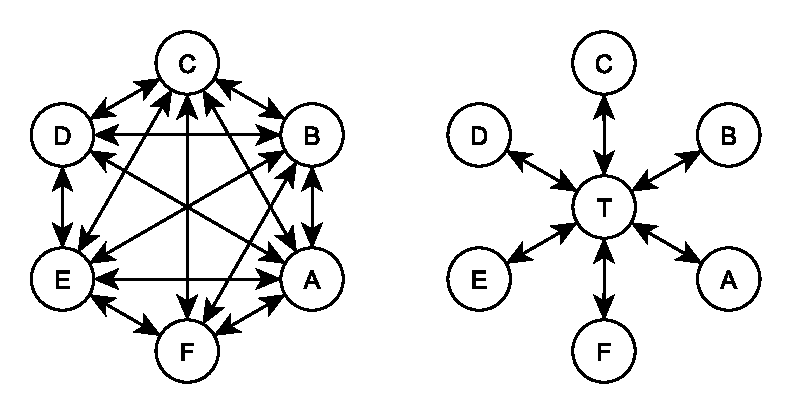
\includegraphics[width=0.8\textwidth]{pic/key_distribution-networks}
    \caption{Варианты сетей без выделенного доверенного центра и с выделенным доверенным центром T\label{fig:key_distribution-networks}}
\end{figure}

Важным моментом при анализе решений данной задачи является то, что сессионные ключи, вырабатываемые в конкретный момент времени, являются менее надёжными, чем мастер-ключи, используемые для генерации сессионных. В частности, нужно предполагать, что хотя злоумышленник не может получить сессионный ключ во время общения абонентов, он может сделать это по прошествии некоторого времени (дни, недели, месяцы). И хотя знание этого сессионного ключа поможет злоумышленнику расшифровать старые сообщения, он не должен иметь возможность организовать новую сессию с использованием уже известного ему сессионного ключа.

\section{Симметричные протоколы}
\selectlanguage{russian}

Как отмечено ранее в разделе~\ref{section-protocols-classification} про классификацию протоколов, к симметричным будем относить те протоколы, которые используют примитивы только классической криптографии на секретных ключах. К ним относятся уже известные блочные шифры, криптографически стойкие генераторы псевдослучайных чисел (КСГПСЧ) и хэш-функции.

\subsection{Протокол Wide-Mouth Frog}\index{протокол!Wide-Mouth Frog|(}
Протокол Wide-Mouth Frog является, возможно, самым простым протоколом с доверенным центром. Его автором считается Майкл Бэрроуз (1989 год, \langen{Michael Burrows},  \cite{Burrows:Abadi:Needham:1990}). Протокол состоит из следующих шагов.

\begin{figure}[!htb]
    \centering
    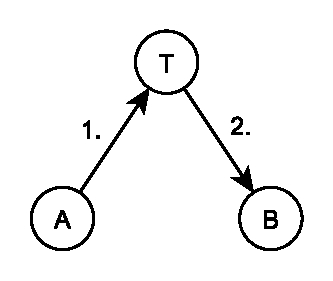
\includegraphics[width=0.5\textwidth]{pic/key_distribution-wide-mouth_frog}
    \caption{Схема взаимодействия абонентов и доверенного центра в протоколе Wide-Mouth Frog\label{fig:key_distribution-wide-mouth_frog}}
\end{figure}

\begin{enumerate}
	\item Алиса генерирует новый сеансовый ключ $K$ и отправляет его вместе с меткой времени, идентификатором Боба и своим незашифрованным идентификатором доверенному центру:
	\[ Alice \rightarrow \{ A, E_A \left( T_A, B, K \right) \} \rightarrow Trent \]
	\item Доверенный центр, используя полученный незашифрованный идентификатор $A$, находит у себя в базе данных легальных абонентов секретный ключ Алисы и расшифровывает им пакет данных. Проверяет метку времени (что пакет не очень старый). Далее он отправляет похожий пакет данных Бобу, зашифрованный его секретным ключом:
	\[ Trent \rightarrow \{ E_B \left( T_T, A, K \right) \} \rightarrow Bob \]
	Боб, кроме расшифрования пакета, также проверяет метку времени доверенного центра.
\end{enumerate}

По окончании протокола у Алисы и Боба есть общий сеансовый ключ $K$.

У данного протокола множество недостатков.

\begin{itemize}
	\item Генератором ключа является инициирующий абонент. Если предположить, что Боб -- это сервер, предоставляющий некоторый сервис, а Алиса -- это тонкий клиент, запрашивающий данный сервис, получается, что задача генерации надёжного сессионного ключа взваливается на плечи абонента с наименьшими мощностями.
	\item В протоколе общение с вызываемым абонентом происходит через доверенный центр. Как следствие, второй абонент может стать мишенью для DDOS-атаки с отражением (\langen{distributed denial-of-service attack}), когда злоумышленник будет посылать пакеты на доверенный центр, а тот формировать новые пакеты и посылать их абоненту. Если абонент подключён к нескольким сетям (с несколькими доверенными центрами), это позволит злоумышленнику вывести абонента из строя. Хотя защититься от подобной атаки достаточно просто, настроив соответствующим образом доверенный центр.
\end{itemize}

Однако самой серьёзной проблемой протокола является возможность применения следующих атак.

В 1995 году Рос Андерсон и Роджер Нидхем (\langen{Ross Anderson, Roger Needham}, \cite{Anderson:Needham:1995}) предложили вариант атаки на протокол, при котором злоумышленник (Ева) может бесконечно продлевать срок действия конкретного сеансового ключа. Идея атаки в том, что после окончания протокола злоумышленник будет посылать доверенному центру назад его же пакеты, дополняя их идентификаторами якобы инициирующего абонента.

\begin{enumerate}
	\item $ Alice \rightarrow \{ A, E_A \left( T_A, B, K \right) \} \rightarrow Trent $
	\item $ Trent \rightarrow \{ E_B \left( T_T, A, K \right) \} \rightarrow Bob $
	\item $ Eva \rightarrow \{ B, E_B \left( T_A, A, K \right) \} \rightarrow Trent $
	\item $ Trent \rightarrow \{ E_A \left( T'_T, B, K \right) \} \rightarrow Alice $
	\item $ Eva \rightarrow \{ A, E_A \left( T'_T, B, K \right) \} \rightarrow Trent $
	\item $ Trent \rightarrow \{ E_B \left( T''_T, A, K \right) \} \rightarrow Bob $
	\item Повторять шаги 3 и 5, пока не пройдёт время, нужное для получения $K$.
\end{enumerate}

С точки зрения доверенного центра, шаги 1, 3 и 5 являются корректными пакетами, инициирующими общение абонентов между собой. Метки времени в них корректны (если Ева будет успевать вовремя эти пакеты посылать). С точки зрения легальных абонентов каждый из пакетов является приглашением другого абонента начать общение. В результате произойдёт две вещи:

\begin{itemize}
	\item Каждый из абонентов будет уверен, что закончился протокол создания нового сеансового ключа, что второй абонент успешно аутентифицировал себя перед доверенным центром. И что для установления следующего сеанса связи будет использоваться новый (на самом деле -- старый) ключ $K$.
	\item После того, как пройдёт время, нужное злоумышленнику Еве для взлома сеансового ключа $K$, Ева сможет и читать всю переписку, проходящую между абонентами, и успешно выдавать себя за обоих из абонентов.
\end{itemize}

Вторая атака 1997 года Гэвина Лоу (\langen{Gavin Lowe}, \cite{Lowe:1997}) проще в реализации. В результате этой атаки Боб уверен, что Алиса аутентифицировала себя перед доверенным центром и хочет начать второй сеанс общения. Что, конечно, не является правдой, так как второй сеанс инициирован злоумышленником.

\begin{enumerate}
	\item $ Alice \rightarrow \{ A, E_A \left( T_A, B, K \right) \} \rightarrow Trent $
	\item $ Trent \rightarrow \{ E_B \left( T_T, A, K \right) \} \rightarrow Bob $
	\item $ Eva \rightarrow \{ E_B \left( T_T, A, K \right) \} \rightarrow Bob $
\end{enumerate}

В той же работе Лоу предложил модификацию протокола, вводящую явную взаимную аутентификацию абонентов с помощью случайной метки $R_B$ и проверки, что Алиса может расшифровать пакет с меткой, зашифрованной общим сеансовым ключом абонентов $K$. Однако данная модификация приводит к тому, что протокол теряет своё самое главное преимущество перед другими протоколами -- простоту.

\begin{enumerate}
	\item $ Alice \rightarrow \{ A, E_A \left( T_A, B, K \right) \} \rightarrow Trent $
	\item $ Trent \rightarrow \{ E_B \left( T_T, A, K \right) \} \rightarrow Bob $
	\item $ Bob \rightarrow \{ E_K \left( R_B \right) \} \rightarrow Alice $
	\item $ Alice \rightarrow \{ E_K \left( R_B + 1 \right) \} \rightarrow Bob $
\end{enumerate}

\index{протокол!Wide-Mouth Frog|)}


\subsection{Протокол Нидхема~---~Шрёдера}\index{протокол!Нидхема~---~Шрёдера|(}\label{section-protocols-needham-schroeder}
\selectlanguage{russian}

Протокол Нидхема~---~Шрёдера (\langen{Roger Needham, Michael Shroeder}, 1979,~\cite{Needham:Schroeder:1978}) похож на модифицированный протокол Wide-Mouth Frog, но отличается тем, что доверенный центр (Трент) во время работы основной части протокола не общается со вторым абонентом. Первый абонент получает от доверенного центра специальный пакет, который он без всякой модификации отправляет второму абоненту.

\begin{figure}[!htb]
    \centering
    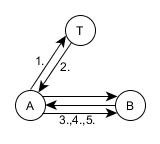
\includegraphics[width=0.5\textwidth]{pic/key_distribution-needham-schroeder}
    \caption{Схема взаимодействия абонентов и доверенного центра в протоколе Нидхема~---~Шрёдера\label{fig:key_distribution-needham-schroeder}}
\end{figure}

\begin{enumerate}
	\item $ Alice	\rightarrow \{ A, B, R_A \}						\rightarrow Trent $
	\item $ Trent	\rightarrow \{ E_A \left( R_A, B, K, E_B \left( K, A \right) \right) \}	\rightarrow Alice $
	\item $ Alice	\rightarrow \{ E_B \left( K, A \right) \}				\rightarrow Bob $
	\item $ Bob	\rightarrow \{ E_K \left( R_B \right) \}				\rightarrow Alice $
	\item $ Alice	\rightarrow \{ E_K \left( R_B - 1 \right) \}				\rightarrow Bob $
\end{enumerate}

Протокол обеспечивает и двустороннюю аутентификацию сторон, и, казалось бы, защиту от атак с повторной передачей (\langen{replay attack}). Последнее делается с помощью введения уже известных по модифицированному протоколу Wide-Mouth Frog случайных меток $R_A$ и $R_B$. Действительно, без знания ключа злоумышленник не сможет выдать себя за Алису перед Бобом (так как не сможет расшифровать пакет с зашифрованной меткой $R_B$). Однако, как мы договорились ранее во введении к этой главе, сам сессионный ключ не может считаться надёжным длительное время. Если злоумышленник сумеет в какой-то момент времени получить ранее использованный сессионный ключ $K$, он сможет убедить Боба, что он является Алисой, и что это новый сессионный ключ. Для этого ему понадобится переданный ранее по открытому каналу пакет из пункта 3 протокола.

\begin{enumerate}
	\item $ Eva		\rightarrow \{ A, B, R_A \}						\rightarrow Trent $
	\item $ Trent		\rightarrow \{ E_A \left( R_A, B, K, E_B \left( K, A \right) \right) \}	\rightarrow Alice $
	\item $ Alice		\rightarrow \{ E_B \left( K, A \right) \}				\rightarrow Bob $
	\item $ Bob		\rightarrow \{ E_K \left( R_B \right) \}				\rightarrow Alice $
	\item $ Alice		\rightarrow \{ E_K \left( R_B - 1 \right) \}				\rightarrow Bob $

		$\dots$ по прошествии некоторого времени $\dots$\\
	\item $ Eva~(Alice)	\rightarrow \{ E_B \left( K, A \right) \}				\rightarrow Bob $
	\item $ Bob		\rightarrow \{ E_K \left( R_B \right) \}				\rightarrow Eva~(Alice) $
	\item $ Eva (Alice)	\rightarrow \{ E_K \left( R_B - 1 \right) \}				\rightarrow Bob $
\end{enumerate}

Относительно мелкий недостаток протокола состоит ещё и в том, что во втором пакете доверенный центр в зашифрованном виде передаёт то, что в третьем шаге пересылается по открытому каналу ($E_B \left( K, A \right)$).

Если в протокол добавить метки времени, тем самым ограничив время возможного использования сессионного ключа, а также исправить мелкий недостаток с двойным шифрованием, можно получить протокол, который лежит в основе распространённого средства аутентификации <<Kerberos>> для локальных сетей.

\index{протокол!Нидхема~---~Шрёдера|)}


\subsection{Протокол <<Kerberos>>}\index{протокол!Kerberos|(}
\selectlanguage{russian}

В данном разделе будет описан протокол аутентификации сторон с единственным доверенным центром. Сетевой протокол <<Kerberos>> использует эти идеи при объединении нескольких доверенных центров в единую сеть для обеспечения надёжности и отказоустойчивости. Подробнее о сетевом протоколе <<Kerberos>> смотрите в разделе~\ref{section-kerberos}.

Как и в протоколе Нидхема~---~Шрёдера, инициирующий абонент (Алиса) общается только с выделенным доверенным центром, получая от него два пакета с зашифрованным сессионным ключом -- один для себя, а второй -- для вызываемого абонента (Боба). Однако в отличие от Нидхема~---~Шрёдера в рассматриваемом протоколе зашифрованные пакеты содержат также метку времени $T_T$ и срок действия сессионного ключа $L$ (от \langen{lifetime} -- срок жизни). Что позволяет, во-первых, защититься от рассмотренной в предыдущем разделе атаки повтором. А, во-вторых, позволяет доверенному центру в некотором смысле управлять абонентами, заставляя их получать новые сессионные ключи по истечению заранее заданного времени $L$.

\begin{figure}[!htb]
    \centering
    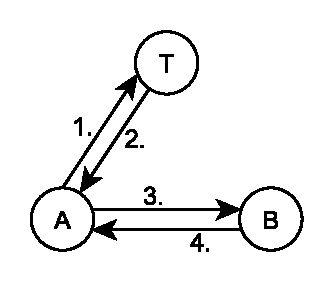
\includegraphics[width=0.5\textwidth]{pic/key_distribution-kerberos}
    \caption{Схема взаимодействия абонентов и доверенного центра в протоколе <<Kerberos>>\label{fig:key_distribution-kerberos}}
\end{figure}

\begin{enumerate}
	\item $ Alice	\rightarrow \{ A, B \}									\rightarrow Trent $
	\item $ Trent	\rightarrow \{ E_A \left( T_T, L, K, B \right), E_B \left( T_T, L, K, A \right) \}	\rightarrow Alice $
	\item $ Alice	\rightarrow \{ E_B \left( T_T, L, K, A \right), E_K \left( A, T_A \right) \}		\rightarrow Bob $
	\item $ Bob	\rightarrow \{ E_K \left( T_T + 1 \right) \}						\rightarrow Alice $
\end{enumerate}

Обратите внимание, что третий шаг за счёт использования метки времени от доверенного центра $T_T$ вместо случайной метки от Боба $R_B$ позволяет сократить протокол на один шаг по сравнению с протоколом Нидхема~---~Шрёдера. Также наличие метки времени делает ненужным и предварительную генерацию случайной метки Алисой и её передачу на первом шаге.

Интересно отметить, что пакеты $E_A \left( T_T, L, K, B \right)$ и $E_B \left( T_T, L, K, A \right)$ одинаковы по своему формату. В некотором смысле их можно назвать сертификатами сессионного ключа для Алисы и Боба. Причём все подобные пары пакетов можно сгенерировать заранее (например, в начале дня), выложить на общедоступный ресурс, предоставить в свободное использование и выключить доверенный центр (он своё дело уже сделал -- сгенерировав эти пакеты). И до момента времени $T_T + L$ этими <<сертификатами>> можно пользоваться. Но только если вы являетесь одной из допустимых пар абонентов. Конечно, эта идея непрактична -- ведь количество таких пар растёт как квадрат от числа абонентов. Однако интересен тот факт, что подобные пакеты можно сгенерировать заранее. Эта идея нам пригодится при рассмотрении инфраструктуры открытых ключей (\langen{public key infrastructure, PKI}).

\index{протокол!Kerberos|)}


\section{Трёхпроходные протоколы}
\selectlanguage{russian}

Если между Алисой и Бобом существует канал связи, недоступный для модификации злоумышленником (то есть когда применима модель только пассивного криптоаналитика), то даже без предварительного обмена секретными ключами или другой информацией можно воспользоваться идеями, использованными ранее в криптографии на открытых ключах. После описания RSA в 1978 году, в 1980 Ади Шамир предложил использовать криптосистемы, основанные на коммутативных операциях, для передачи информации без предварительного обмена секретными ключами. Если предположить, что передаваемой информацией является выработанный одной из сторон секретный сеансовый ключ, то в общем виде мы получаем следующий трёхпроходной протокол.

Предварительно:

\begin{itemize}
	\item Алиса и Боб соединены незащищённым каналом связи, открытым для прослушивания (но не для модификации) злоумышленником.
	\item Каждая из сторон имеет пару из открытого и закрытого ключей $K_A$, $k_A$, $K_B$, $k_B$ соответственно.
	\item Сторонами выбрана и используется коммутативная функция шифрования:
	\begin{align*}
		D_{A} \left( E_{A} \left( X \right) \right)	&= X		& ~~\forall ~ X, \left\{ K_A, k_a \right\}; \\
		E_{A} \left( E_{B} \left( X \right) \right)	&= E_B \left( E_A \left( X \right) \right) & ~~\forall ~ K_A, K_B, X.
	\end{align*}
\end{itemize}

Протокол состоит из трёх шагов (отсюда и название).
\begin{enumerate}
    \item Алиса создаёт новый секретный сеансовый ключ $K_S$, шифрует его с помощью своего ключа $K_A$ и посылает сообщение Бобу:
        \[ Alice \rightarrow ~ E_A \left( K_S \right) ~ \rightarrow Bob. \]
    \item Боб получает это сообщение, шифрует его с помощью своего ключа $K_B$ и посылает сообщение Алисе:
        \[ Bob \rightarrow ~ E_B \left( E_A \left( K_S \right) \right) ~ \rightarrow Alice. \]
    Алиса, получив сообщение $E_B \left( E_A \left( K_S \right) \right)$, использует свой закрытый ключ $k_A$ для расшифрования:
	\[ D_A \left( E_B \left( E_A \left( K_S \right) \right) \right) = D_A \left( E_A \left( E_B \left( K_S \right) \right) \right) = E_B \left( K_S \right). \]
    \item Алиса передаёт Бобу сообщение, в котором новый секретный сеансовый ключ зашифрован уже только ключом Боба:
        \[ Alice \rightarrow ~ E_B \left( K_S \right) ~ \rightarrow Bob. \]
    Боб, получив сообщение $E_B \left( K_S \right)$, использует свой ключ $k_B$ для расшифрования:
	\[ D_B \left( E_B \left( K_S \right) \right) = K_S. \]
\end{enumerate}

В результате стороны получают общий секретный ключ $K_S$.

Общим недостатком всех подобных протоколов является отсутствие аутентификации сторон. Конечно, в случае пассивного криптоаналитика это не требуется, но в реальной жизни всё-таки нужно рассматривать все возможные модели (в том числе активного криптоаналитика) и использовать такие протоколы, которые предполагают взаимную аутентификацию сторон.

\subsection{Тривиальный вариант}

Приведём пример протокола на основе функции XOR (побитовое сложение по модулю 2). Хотя данная функция может использоваться как фундамент для построения систем совершенной криптостойкости (см. главу~\ref{chapter:perfect_secure_systems}), для трёхпроходного протокола это неудачный выбор.

Перед началом протокола обе стороны имеют свои секретные ключи $K_A$ и $K_B$, представляющие собой случайные двоичные последовательности с равномерным распределением символов. Функция шифрования определяется как $E_i( X ) = X \oplus K_i$, где $X$ это сообщение, а $K_i$ -- секретный ключ. Очевидно, что:
\[ \forall i, j, X: E_i \left( E_j \left( X \right) \right) = X \oplus K_j \oplus K_i = X \oplus K_i \oplus K_j = E_j \left( E_i \left( X \right) \right) \]

\begin{enumerate}
    \item Алиса генерирует новый сеансовый ключ, шифрует его своим секретным ключом $K_A$ и посылает Бобу:
            \[\begin{array}{l}
		E_A(K) = K \oplus K_A, \\
		Alice \rightarrow ~ E_A(K) ~ \rightarrow Bob.
	    \end{array}\]
    \item Боб шифрует полученное сообщение уже своим ключом и отправляет Алисе:
            \[\begin{array}{l}
		E_B(E_A(K)) = K \oplus K_A \oplus K_B, \\
		Bob \rightarrow ~ E_B(E_A(K)) ~ \rightarrow Alice.
	    \end{array}\]
    \item Используя коммутативность операции шифрования, Алиса <<снимает>> шифрование своим ключом и отправляет результат Бобу:
            \[ D_A \left( E_B \left( E_A \left( K \right) \right) \right) = K \oplus K_A \oplus K_B \oplus K_A = K \oplus K_B = E_B \left( K \right). \]
            \[ Alice \rightarrow ~ E_B \left( K \right) ~ \rightarrow Bob. \]
    Боб, получив сообщение $K \oplus K_B$, выполняет расшифрование:
            \[ D_B( E_B( K ) ) = K \oplus K_B \oplus K_B = K. \]
    В результате Алиса и Боб знают общий сеансовый ключ $K$.
\end{enumerate}

Предложенный выбор коммутативной функции шифрования совершенной секретности был назван неудачным, так как существуют ситуации, при которых криптоаналитик может определить ключ $K$. Предположим, что криптоаналитик перехватил все три сообщения:
    \[ K \oplus K_A, ~~ K \oplus K_A \oplus K_B, ~~ K \oplus K_B. \]
Сложение по модулю 2 всех трёх сообщений даёт ключ $K$. Поэтому такая система шифрования не применяется.

Теперь приведём протокол надёжной передачи секретного ключа, основанный на экспоненциальной (коммутативной) функции шифрования. Стойкость этого протокола связана с трудностью задачи вычисления дискретного логарифма: при известных значениях $y, g, p$, найти $x$ из уравнения $y = g^x \mod p$.

\subsection{Бесключевой протокол Шамира}\index{протокол!Шамира бесключевой|(}\label{section-protocols-shamir}

Стороны предварительно договариваются о большом простом числе $p \sim 2^{1024}$. Каждая из сторон выбирает себе по секретному ключу $a$ и $b$. Эти ключи меньше и взаимно просты с $p-1$. Также стороны приготовили по специальному числу $a'$ и $b'$, которые позволяют им расшифровать сообщение, зашифрованное своим ключом:
\[\begin{array}{l}
a' = a{-1} \mod (p-1), \\
a \times a' = 1 \mod (p-1), \\
\forall X: (X^a)^{a'} = X. \\
\end{array}\]

Последнее выражение верно по следствию из малой теоремы Ферма\index{теорема!Ферма малая}. Операции шифрования и расшифрования определяются следующим образом (на примере Алисы):
\[\begin{array}{ll}
\forall X < p:	& E_A( X ) = X^{a} \mod p, \\
		& D_A( X ) = X^{a'} \mod p, \\
		& D_A( E_A( X ) ) = X^{aa'} = X \mod p. \\
\end{array}\]

\begin{enumerate}
    \item Алиса создаёт новый сеансовый ключ $K < p$, шифрует его своим секретным ключом $a$ и посылает сообщение Бобу:
            \[\begin{array}{l}
		E_A(K) = K ^ a \mod p, \\
		Alice \rightarrow ~ E_A(K) ~ \rightarrow Bob.
	    \end{array}\]
    \item Боб шифрует полученное сообщение уже своим ключом и отправляет Алисе:
            \[\begin{array}{l}
		E_B(E_A(K)) = K^{ab} \mod p, \\
		Bob \rightarrow ~ E_B(E_A(K)) ~ \rightarrow Alice.
	    \end{array}\]
    \item Используя коммутативность операции шифрования, Алиса <<снимает>> шифрование своим ключом и отправляет результат Бобу:
            \[ D_A \left( E_B \left( E_A \left( K \right) \right) \right) = \left( K^{ab} \right) ^{a'} = K^{aa'b} = K^{b} = E_B \left( K \right) \mod p. \]
            \[ Alice \rightarrow ~ E_B \left( K \right) ~ \rightarrow Bob. \]
    Боб, получив сообщение $K \oplus K_B$, выполняет расшифрование:
            \[ D_B( E_B( K ) ) = K \oplus K_B \oplus K_B = K. \]
    В результате Алиса и Боб знают общий сеансовый ключ $K$.
\end{enumerate}

Предположим, что криптоаналитик перехватил три сообщения:
\[ \begin{array}{l}
    y_1 = K^a \mod p, \\
    y_2 = K^{ab} \mod p, \\
    y_3 = K^b \mod p. \\
\end{array} \]

Чтобы найти ключ $K$, криптоаналитику надо решить систему из этих трёх уравнений, что имеет очень большую вычислительную сложность, неприемлемую с практической точки зрения, если все три числа $a, b, ab$ достаточно велики. Предположим, что $a$ (или $b$) мало. Тогда, вычисляя последовательные степени $y_3$ (или $y_1$), можно найти $a$ (или $b$), сравнивая результат с $y_2$. Зная $a$, легко найти $a^{-1}\mod(p-1)$ и $K=(y_1)^{a^{-1}}\mod p$.

\index{протокол!Шамира бесключевой|)}

\subsection{Криптосистема Мэсси~---~Омуры}\index{протокол!Мэсси~---~Омуры|(}\index{криптосистема!Мэсси~---~Омуры|(}

В 1982 году Джеймс Мэсси и Джим Омура заявили патент (\langen{James Massey, Jim K. Omura},~\cite{Massey:Omura:1986}), улучшающий (по их мнению) бесключевой протокол Шамира. В качестве операции шифрования вместо возведения в степень в мультипликативной группе $\Z_p^*$ они предложили использовать возведение в степень в поле Галуа $\GF{2^n}$. Секретный ключ каждой стороны (для Алисы -- $a$) должен удовлетворять условиям:
\[ \begin{array}{l}
 a \in \GF{2^n}, \\
 gfd \left( a, x^{ n-1 } + x^{ n-2 } + ... + x + 1 \right) = 1. \\
\end{array} \]

В остальном протокол выглядит аналогично.

\index{протокол!Мэсси~---~Омуры|)}\index{криптосистема!Мэсси~---~Омуры|)}

\section{Асимметричные протоколы}
\selectlanguage{russian}

Асимметричные протоколы, или же протоколы, основанные на криптосистемах с открытыми ключами, позволяют ослабить требования к предварительному этапу протоколов. Вместо общего секретного ключа, который должны иметь две стороны (либо обе стороны и доверенный центр), в рассматриваемых ниже протоколах стороны должны предварительно обменяться открытыми ключами (между собой либо между собой и доверенным центром). Такой предварительный обмен может проходить по открытому каналу связи, в предположении, что криптоаналитик не может повлиять на содержимое канала связи на данном этапе.

\subsection{Простой протокол}

Рассмотрим протокол распространения ключей с помощью асимметричных шифров. Введём обозначения: $K_B$ -- открытый ключ стороны $B$, а $K_A$ -- открытый ключ стороны $A$. Протокол включает три сеанса обмена информацией.
\begin{enumerate}
    \item В первом сеансе сторона $A$ посылает стороне $B$ сообщение:
            \[ A \rightarrow B: ~ E_{K_B}(K_1, A), \]
        где $K_1$ -- ключ, выработанный стороной $A$.
    \item Сторона $B$ получает $(K_1, A)$ и передаёт стороне $A$ наряду с другой информацией свой ключ $K_2$ в сообщении, зашифрованном с помощью открытого ключа $K_A$:
            \[ A \leftarrow B: ~ E_{K_A}(K_2, K_1, B). \]
    \item Сторона $A$ получает и расшифровывает сообщение $(K_2, K_1, B)$. Во время третьего сеанса сторона $A$, чтобы подтвердить, что она знает ключ $K_2$, посылает стороне $B$ сообщение:
            \[ A \rightarrow B: ~ E_{K_B}(K_2). \]
\end{enumerate}
Общий ключ формируется из двух ключей: $K_1$ и $K_2$.

\subsection{Протоколы с цифровыми подписями}

Существуют протоколы обмена, в которых перед началом обмена ключами генерируются подписи сторон $A$ и $B$, соответственно $S_A(m)$ и $S_B(m)$. В этих протоколах можно использовать различные одноразовые метки. Рассмотрим пример.
\begin{enumerate}
    \item Сторона $A$ выбирает ключ $K$ и вырабатывает сообщение:
            \[ \left( K, ~ t_A, ~ S_A(K, t_A, B) \right), \]
        где $t_A$ -- метка времени. Зашифрованное сообщение передаёт стороне $B$:
        \[ A \rightarrow B: ~ E_{K_B}(K, ~ t_A, ~ S_A(K, t_A, B)). \]
    \item Сторона $B$ получает это сообщение, расшифровывает $\left( K, ~ t_A, ~ S_A(K, t_A, B) \right)$ и вырабатывает свою метку времени $t_B$. Проверка считается успешной, если $|t_B - t_A | < \delta $. Сторона $B$ знает свои реквизиты и может осуществлять проверку подписи.
\end{enumerate}

Имеется второй вариант протокола, в котором шифрование и подпись выполняются раздельно.
\begin{enumerate}
    \item Сторона $A$ вырабатывает ключ $K$, использует одноразовую метку (или метку времени) $t_{A}$ и передаёт стороне $B$ два различных зашифрованных сообщения:
            \[ \begin{array}{ll}
                A \rightarrow B: & ~ E_{K_B}(K, t_A), \\
                A \rightarrow B: & ~ S_A(K, t_A, B). \\
            \end{array} \]
    \item Сторона $B$ получает это сообщение, расшифровывает $K, t_A$ и, добавив свои реквизиты, может проверить подпись $S_A(K, t_A, B)$.
\end{enumerate}

В третьем варианте протокола сначала производится шифрование, потом подпись.
\begin{enumerate}
    \item Сторона $A$ вырабатывает ключ $K$, использует одноразовую случайную метку или метку времени $t_A$ и передаёт стороне $B$ сообщение:
        \[ A \rightarrow B: ~ t_A, ~ E_{K_B}(K, A), ~ S_A(t_A, ~ K, ~ E_{K_B}(K, A)). \]
    \item Сторона $B$ получает это сообщение, расшифровывает $\left( K, ~ A \right)$ и проверяет подпись $S_A(t_A, ~ K, ~ E_{K_B}(K, A))$.
\end{enumerate}

\subsection{Протокол Диффи~---~Хеллмана}\index{протокол!Диффи~---~Хеллмана}
\selectlanguage{russian}

Алгоритм с открытым ключом впервые был предложен Диффи и Хеллманом в работе 1976 года <<Новые направления в криптографии>> (\langen{Bailey Whitfield Diffie, Martin Edward Hellman, ``New directions in cryptography''},~\cite{Diffie:Hellman:1976}).

Рассмотрим протокол Диффи~---~Хеллмана обмена информацией двух сторон $A$ и $B$. Задача состоит в том, чтобы создать общий сеансовый ключ.

Пусть $p$ -- большое простое число\index{число!простое}, $g$ -- примитивный элемент группы $\Z_p^*$, ~ $y = g^x \mod p$, причём $p,y,g$ известны заранее. Функцию $y=g^{x} \mod p$ считаем однонаправленной, то есть вычисление функции при известном значении аргумента является лёгкой задачей, а её обращение (нахождение аргумента) при известном значении функции -- трудной.

Протокол обмена состоит из следующих действий.
\begin{enumerate}
    \item Сторона $A$ выбирает случайное число $x: ~ 2 \leq x \leq p-1$, вычисляет и передаёт стороне $B$ сообщение:
        \[ A \rightarrow B: ~ g^x \mod p. \]
    \item Сторона $B$ выбирает случайное число $y: ~ 2\leq y \leq p-1$, вычисляет и передаёт стороне $A$:
        \[ A \leftarrow B: ~ g^y \mod p. \]
    \item Сторона $A$, используя известные ей значения $x$, $g^{y} \mod p$, вычисляет ключ:
        \[ K_{A} =(g^{y})^{x}\mod p=g^{xy} \mod p. \]
    \item Сторона $B$, используя известные ей значения $y$, $g^{x} \mod p$, вычисляет ключ:
        \[ K_{B} =(g^{x})^{y}\mod p=g^{xy}\mod p. \]
        В результате получаем равенство $K_A = K_B = K$.
\end{enumerate}

Таким способом создан общий секретный сеансовый ключ. В каждом новом сеансе используется этот же протокол для создания нового сеансового ключа.

Рассмотрим протокол Диффи~---~Хеллмана в ситуации, когда имеются три легальных пользователя $A,B,C$.

Каждая из сторон $A,B,C$ вырабатывает случайные числа $x,y,z$ соответственно и держит их в секрете.

\begin{enumerate}
    \item Первый этап обмена информацией аналогичен вышеописанному обмену информацией между двумя сторонами:
        \begin{enumerate}
            \item $A \rightarrow B: ~ g^x \mod p$.
            \item $B \rightarrow C: ~ g^y \mod p$.
            \item $C \rightarrow A: ~ g^z \mod p$.
        \end{enumerate}
    \item Второй этап состоит из передач сообщений:
        \begin{enumerate}
            \item $A \rightarrow B: ~ (g^z)^x = g^{zx} \mod p$.
            \item $B \rightarrow C: ~ (g^x)^y = g^{xy} \mod p$.
            \item $C \rightarrow A: ~ (g^y)^z = g^{yz} \mod p$.
        \end{enumerate}
    \item На завершающем третьем этапе стороны вычисляют:
        \begin{enumerate}
            \item $A: ~ K_A = (g^{yz})^x = g^{xyz} \mod p$.
            \item $B: ~ K_B = (g^{zx})^y = g^{xyz} \mod p$.
            \item $C: ~ K_C = (g^{xy})^z = g^{xyz} \mod p$.
        \end{enumerate}
\end{enumerate}

Как видно из произведённых действий, выработанные сторонами $A, B, C$ ключи совпадают: $K_A = K_B = K_C = K$. Следовательно, создан общий секретный сеансовый ключ $K$ для трёх участников.

Таким же образом можно построить протокол Диффи~---~Хеллмана для любого числа легальных пользователей.

Рассмотрим этот двусторонний протокол с точки зрения криптоаналитика, желающего узнать ключ $K$. Предположим, ему удалось перехватить сообщения $g^{x}\mod p$ и $g^{y}\mod p $. Используя заранее известные данные $g,p $ и эти сообщения, криптоаналитик старается найти хотя бы одно из чисел $(x,y)$, то есть решить задачу дискретного логарифма. В настоящее время эта задача считается вычислительно трудной при обычно выбираемых значениях $p\sim 2^{1024}$.

Существует атака активного криптоаналитика\index{криптоаналитик!активный}, названная <<человек посередине>> (man-in-the-middle)\index{атака!<<человек посередине>>}. Пусть имеются две легальные стороны $A$ и $B$ и нелегальная сторона $E$ -- активный криптоаналитик\index{криптоаналитик!активный}, который имеет возможность перехватывать и подменять сообщения как от $A$, так и от $B$:
    \[ A \leftrightsquigarrow E \leftrightsquigarrow B. \]
    %\[ A \leftrightarrow E \leftrightarrow B. \]

\begin{enumerate}
    \item Подмена ключей.
        \begin{enumerate}
            \item Сторона $A$ передаёт стороне $B$ сообщение:
                \[ A \overset{E}{\nrightarrow} B: ~ g^x \mod p. \]
            \item Сторона $E$ перехватывает сообщение $g^x \mod p$, сохраняет его и, зная $g$, передаёт стороне $B$ своё сообщение:
                \[ E \rightarrow B: ~ g^z \mod p. \]
            \item Сторона $B$ передаёт стороне $A$ сообщение:
                \[ A \overset{E}{\nleftarrow} B: ~ g^y \mod p. \]
            \item Сторона $E$ перехватывает сообщение $g^y \mod p$, сохраняет его и передаёт стороне $A$ своё сообщение:
                \[ A \leftarrow E: ~ g^z \mod p \]
                или какое-то другое.
            \item Таким образом, между сторонами $A$ и $E$ образуется общий секретный ключ $K_{AE}$, между $B$ и $E$ -- ключ $K_{BE}$, причём $A$ и $B$ не знают, что у них ключи со стороной $E$, а не друг с другом:
                \[ \begin{array} {l}
                    K_{AE} = g^{xz} \mod p, \\
                    K_{BE} = g^{yz} \mod p. \\
                \end{array} \]

        \end{enumerate}
    \item Подмена сообщений.
        \begin{enumerate}
            \item Сторона $A$ посылает $B$ сообщение $m$, зашифрованное на ключе $K_{AE}$:
                % \rightsquigarrow
                \[ A \overset{E}{\nrightarrow} B: ~ E_{K_{AE}}(m). \]
            \item Сторона $E$ перехватывает сообщение, расшифровывает с ключом $K_{AE}$, возможно, подменяет на $m'$, зашифровывает с ключом $K_{BE}$ и посылает $B$:
                \[ E \rightarrow B: ~ E_{K_{BE}}(m'). \]
            \item То же самое происходит при обратной передаче от $B$ к $A$.
        \end{enumerate}
\end{enumerate}

Криптоаналитик $E$ имеет возможность перехватывать и подменять все передаваемые сообщения. Если по тексту письма нельзя обнаружить участие криптоаналитика в обмене информацией, то атака <<человек посередине>>\index{атака!<<человек посередине>>} успешна.

Существует несколько протоколов для защиты от атаки этого типа.


%\section{Протоколы с аутентификацией}

\subsection{Односторонняя аутентификация}

\textbf{Протокол Эль-Гамаля}\index{протокол!Эль-Гамаля} относится к протоколам с аутентификацией одного из двух легальных пользователей.
\selectlanguage{russian}
\begin{enumerate}
    \item Для начала стороны выбирают общие параметры $p, g$, где $p$ -- большое простое число, а $g$ -- примитивный элемент поля $\Z_p^*$.
    \item Сторона $B$ создаёт свои закрытый и открытый ключи:
            \[ \SK_B = b, ~ \PK_B = g^b \mod p, \]
        $b$ -- случайное секретное число, $2 \leq b \leq p-1$.

        Открытый ключ $\PK_B$ находится в общем открытом доступе для всех сторон, поэтому криптоаналитик $E$ не может подменить его -- подмена будет заметна.
    \item Сторона $A$ вырабатывает свой секрет $x$, сеансовый ключ
            \[ K_A = (\PK_B)^x = g^{bx} \mod p \]
        и отправляет $B$:
            \[ A \rightarrow B: ~ g^x \mod p. \]
    \item Сторона $B$, получив от $A$ число $g^x \mod p$, использует его и свой секрет $\SK_B = b$, чтобы создать свой ключ
            \[ K_B = (g^x)^{\SK_B} = g^{bx} \mod p, \]
        то есть сеансовые ключи обеих сторон совпадают:
            \[ K_A = K_B = K. \]
\end{enumerate}

Достоинством этого протокола является следующее его свойство. Если ключи $K_A$ и $K_B$ совпали и стороны могут обмениваться информацией, то сторона $A$ аутентифицирует сторону $B$, так как для шифрования она использовала открытый ключ $B$, который не может быть незаметно подменён, и только сторона $B$ может расшифровывать сообщения.

Что касается криптоаналитика в качестве <<человека посередине>>, то он может отправлять ложные сообщения, но не может узнать ключ $K$ и читать сообщения.

Есть протоколы, в которых стороны, осуществляющие обмен информацией, являются равноправными. Они называются протоколами взаимной аутентификации.


\subsection{Взаимная аутентификация шифрованием}
\selectlanguage{russian}

К протоколам взаимной аутентификации принадлежит семейство протоколов, разработанных Ц.~Мацумото (\langen{Tsutomu Matsumoto}), И.~Такашима (\langen{Youichi Takashima}) и Х.~Имаи (\langen{Hideki Imai}) и названных по первым буквам фамилий авторов -- \emph{протоколы MTI}\index{протоколы!MTI}.

Здесь к открытым данным относятся:
    \[ p, ~~ g, ~~ \PK_A = g^a \mod p, ~~ \PK_B = g^b \mod p. \]
Каждый из пользователей $A$ и $B$ обладает парой долговременных ключей для \emph{схемы шифрования с открытым ключом}: закрытым ключом расшифрования $\SK$ и открытым ключом шифрования $\PK$.
\[ \begin{array}{ll}
    A: & ~ \SK_A = a, ~~ \PK_A = g^a \mod p, \\
    B: & ~ \SK_B = b, ~~ \PK_B = g^b \mod p. \\
\end{array} \]

\textbf{Протокол MTI}:
\begin{enumerate}
    \item Сторона $A$ генерирует случайное число $x, ~ 2\leq x\leq p-1$, создаёт и отправляет $B$ сообщение:
        \[ A \rightarrow B: ~ g^x \mod p. \]
    \item Сторона $B$ генерирует случайное число $y, ~ 2\leq y\leq p-1$, создаёт и отправляет $A$ сообщение:
        \[ A \leftarrow B: ~ g^y \mod p. \]
    \item Сторона $A$, используя открытые данные и полученное сообщение, создаёт сеансовый ключ:
        \[ K_A = (g^b)^x \cdot (g^y)^a = g^{bx+ay} \mod p. \]
    \item Сторона $B$, используя открытые данные и полученное сообщение, создаёт сеансовый ключ:
        \[ K_B = (g^x)^b \cdot (g^a)^y = g^{bx+ay} \mod p. \]
        Сеансовые ключи обеих сторон совпадают:
        \[ K_{A} =K_{B} = K. \]
\end{enumerate}

В описанном протоколе, как и в протоколе Эль-Гамаля\index{криптосистема!Эль-Гамаля}, происходит взаимная аутентификация сторон: открытые ключи сторон незаметно подменить невозможно. Наблюдая сообщения протокола, вычислить $g^{bx+ay}$ можно, только если известны значения $a,x$ или $b,y$, что представляет собой задачу дискретного логарифмирования, вычислительно трудную на сегодняшний день.


\subsection{Взаимная аутентификация схемой ЭП}
\selectlanguage{russian}

\emph{Протокол STS (Station-to-Station)}\index{протокол!Station-to-Station} предназначен для систем мобильной связи. Он использует идеи протокола Диффи~---~Хеллмана\index{протокол!Диффи~---~Хеллмана} и криптосистемы RSA\index{криптосистема!RSA}. Особенностью протокола является использование механизма электронной подписи\index{электронная подпись} для взаимной аутентификации сторон\index{аутентификация!взаимная}.

Здесь открытые общедоступные данные:
    \[ p, ~ g, ~ \PK_A, ~ \PK_B. \]

Каждая из сторон $A$ и $B$ обладает долговременной парой ключей: закрытым ключом для создания электронной подписи $\SK$ и открытым ключом для проверки подписи $\PK$:
\[ \begin{array}{ll}
    A: & ~ \SK_A, ~~ \PK_A, \\
    B: & ~ \SK_B, ~~ \PK_B. \\
\end{array} \]

Протокол состоит из трёх раундов обмена информацией между сторонами $A$ и $B$.
\begin{enumerate}
    \item Сторона $A$ создаёт секретное случайное число $x: 2 \leq x \leq p-1$ и отправляет $B$:
            \[ A \rightarrow B: ~ g^x \mod p. \]
    \item Сторона $B$ создаёт секретное случайное число $y: 2 \leq y \leq p-1$, вычисляет общий секретный ключ
            \[ K = (g^x)^y = g^{xy} \mod p, \]
        с помощью которого создаёт шифрованное сообщение $E_K(S_B(g^x, g^y))$ для аутентификации, и отправляет $A$:
            \[ A \leftarrow B: ~ \left( g^y \mod p, ~~ E_K( S_B( g^x, g^y)) \right). \]
    \item Сторона $A$ с помощью $x$, $g^y \mod p$ вычисляет общий секретный ключ
            \[ K = (g^y)^x \mod p = g^{xy} \mod p \]
        и расшифровывает сообщение:
            \[ D_K( E_K( S_B( g^x, g^y))) = S_B( g^x, g^y). \]
            Затем аутентифицирует сторону $B$, проверяя подпись $S_B$ открытым ключом $\PK_B$. Вычисляет и пересылает стороне $B$ сообщение:
            \[ A \rightarrow B: ~ E_K( S_A( g^x, g^y)). \]
    \item Сторона $B$ расшифровывает принятое сообщение:
            \[ D_K( E_K( S_A( g^x, g^y))) = S_A( g^x, g^y) \]
        и осуществляет аутентификацию, выполняя проверку подписи $S_A$ с помощью открытого ключа $\PK_A$.
\end{enumerate}


\subsection{Взаимная аутентификация с доверенным центром}
\selectlanguage{russian}

В \emph{протоколе Жиро}\index{протокол!Жиро} (\langfr{Marc Girault},~\cite{Girault:1990, Girault:1991}) участвуют три стороны -- $A$, $B$ и надёжный центр $T$.
\begin{enumerate}
    \item У стороны $T$ есть открытый и закрытый ключи криптосистемы RSA\index{криптосистема!RSA},
        \[ n=pq, ~ e, ~ d=e^{-1} \mod \varphi(n), \]
        с дополнительным параметром $g$ -- генератором подгруппы максимально возможного порядка мультипликативной группы $\Z_n^*$:
        \[ \begin{array}{l}
            \PK_T = (n, e, g) ~~\text{открытый ключ}, \\
            \SK_T = (d) ~~ \text{закрытый ключ}. \\
        \end{array} \]
    \item Стороны $A$ и $B$ независимо друг от друга создают свои открытые и закрытые ключи, обмениваясь информацией с центром $T$ по надёжному защищённому каналу. Стороны $A$ и $B$ выбирают свои закрытые ключи:
        \[ \begin{array}{l}
            \SK_A = a, \\
            \SK_B = b \\
        \end{array} \]
     и отправляют центру сообщения:
        \[ \begin{array}{ll}
            A \to T: & ~ I_A, ~~ g^{-\SK_A} = g^{-a} \mod n, \\
            B \to T: & ~ I_B, ~~ g^{-\SK_B} = g^{-b} \mod n, \\
        \end{array} \]
        где $I_A, I_B$ -- числовые идентификаторы сторон.
    \item Центр $T$ вычисляет открытые ключи для $A$ и $B$ и также по надёжному каналу передаёт им:
        \[ \begin{array}{ll}
            A \leftarrow T: & ~ \PK_A = (g^{-\SK_A} - I_A)^{\SK_T} = (g^{-a} - I_A)^d \mod n, \\
            B \leftarrow T: & ~ \PK_B = (g^{-\SK_B} - I_B)^{\SK_T} = (g^{-b} - I_B)^d \mod n. \\
        \end{array} \]
    \item Теперь стороны $A$ и $B$ могут создать общий секретный симметричный сеансовый ключ. Например, $A$ находит:
        \[ \begin{array}{ll}
            A: ~~ K_A & = ~ (\PK_B^e + I_B)^{\SK_A} ~ = \\
                & = ~ (((g^{-b} - I_B)^d)^e + I_B)^a ~ = \\
                & = ~ (g^{-b} - I_B + I_B)^a ~ = \\
                & = ~ g^{-ab} \mod n. \\
        \end{array} \]
        Аналогично $B$ вычисляет:
            \[ K_B = (\PK_A^e + I_A)^{\SK_B} = g^{-ab} \mod n. \]
        Как видно, ключи одинаковы:
            \[ K = K_A = K_B = g^{-ab} \mod n. \]
\end{enumerate}


\subsection{Схема Блома}\label{section-bloms-scheme}\index{схема!Блома|(}
\selectlanguage{russian}

Схема Блома (\langen{Rolf Blom},~\cite{Blom:1984, Blom:1985}) используется в протоколе HDCP\index{протокол!HDCP} (\langen{High-bandwidth Digital Content Protection}) для предотвращения копирования высококачественного видеосигнала. Предполагается, что некоторый доверенный центр распределит ключи таким образом, что легальные производители видеокарт, мониторов высокого разрешения и других компонент будут передавать видеоконтент по защищённому каналу, а <<пиратские>> устройства не смогут эти данные перехватить, и, например, записать на другой носитель.

На этапе инициализации доверенный центр выбирает симметричную матрицу $D_{m,m}$ над конечным полем $\GF p$. Для присоединения к сети распространения ключей, новый участник либо самостоятельно, либо с помощью доверенного центра выбирает новый открытый ключ (идентификатор) $I_i$, представляющий собой вектор длины $m$ над $\GF p$. Доверенный центр вычисляет для нового участника закрытый ключ $K_i$:
\begin{equation}
	K_i = D_{m,m} I_i.
	\label{eq:blom_center_matrix}
\end{equation}

Симметричность матрицы $D_{m,m}$ доверенного центра позволяет любым двум участникам сети создать общий сеансовый ключ. Пусть Алиса и Боб -- легальные пользователи сети, то есть они обладают открытыми ключами $I_A$ и $I_B$ соответственно, а их закрытые ключи $K_A$ и $K_B$ были вычислены одним и тем же доверенным центром по формуле~\ref{eq:blom_center_matrix}. Тогда протокол выработки общего секретного ключа выглядит следующим образом (рис.~\ref{fig:key_distribution-bloms-scheme}).

\begin{figure}
    \centering
    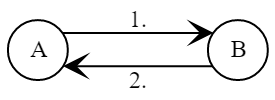
\includegraphics[width=0.5\textwidth]{pic/key_distribution-bloms-scheme}
    \caption{Взаимодействие участников в схеме Блома\label{fig:key_distribution-bloms-scheme}}
\end{figure}

\begin{protocol}
    \item[(1)] $Alice \to \left\{ I_A \right\} \to Bob$
    \item[(2)] Боб вычисляет $K_{BA} = K^T_B I_A = I^T_B D_{m,m} I_A$.
    \item[{}] $Bob \to \left\{ I_B \right\} \to Alice$
    \item[(3)] Алиса вычисляет $K_{AB} = K^T_A I_B = I^T_A D_{m,m} I_B$.
\end{protocol}

Из симметричности матрицы $D_{m,m}$ следует, что значения $K_{AB}$ и $K_{BA}$ совпадут, они же и будут являться общим секретным ключом для Алисы и Боба. Этот секретный ключ будет свой для каждой пары легальных пользователей сети.

Присоединение новых участников к схеме строго контролируется доверенным центром, что позволяет защитить сеть от нелегальных пользователей. Надёжность данной схемы основывается на невозможности восстановить исходную матрицу. Однако для восстановления матрицы доверенного центра размера $m \times m$ необходимо и достаточно всего $m$ пар линейно независимых открытых и закрытых ключей. В 2010-м году компания Intel, которая является <<доверенным центром>> для пользователей системы защиты HDCP, подтвердила, что криптоаналитикам удалось найти секретную матрицу (точнее, аналогичную ей), используемую для генерации ключей в упомянутой системе предотвращения копирования высококачественного видеосигнала.

\index{схема!Блома|)}


\section{Квантовые протоколы}\index{протокол!квантовые|(}

\subsection{Протокол BB84}\index{протокол!BB84|(}
\selectlanguage{russian}

В 1984 году Чарльз Беннетт (\langen{Charles Henry Bennett}) и Жиль Брассар (\langfr{Gilles Brassard}) предложили новый квантовый протокол распределения ключа~\cite{Bennett:Brassard:1984}. Как и у других протоколов, его целью является создание нового сеансового ключа, который в дальнейшем можно использовать в классической симметричной криптографии. Однако особенностью протокола является использование отдельных положений квантовой физики для гарантии защиты получаемого ключа от перехвата злоумышленником.

До начала очередного раунда генерации сеансового ключа предполагается, что у Алисы и Боба, как у участников протокола, имеется:

\begin{itemize}
	\item квантовый канал связи (например, оптоволокно);
	\item классический канал связи.
\end{itemize}

Протокол гарантирует, что вмешательство злоумышленника в протокол можно заметить вплоть до тех пор, пока злоумышленник не сможет контролировать и чтение, и запись на всех каналах общения сразу.

Протокол состоит из следующих этапов:

\begin{itemize}
	\item передача Алисой и приём Бобом фотона по квантовому каналу связи;
	\item передача Бобом информации об использованных анализаторах;
	\item передача Алисой информации о совпадении выбранных анализаторов и исходных поляризаций.
\end{itemize}


\subsubsection{Генерация фотона}

В первой части протокола, с точки зрения физика-экспериментатора, Алиса берёт единичный фотон и поляризует под одним из четырёх углов: 0, 45, 90 или 135. Будем говорить, что Алиса сначала выбрала базис поляризации (<<+>> или <<x>>), а затем выбрала в этом базисе одно из двух направлений поляризации:

\begin{itemize}
	\item $0^{\circ}$ (<<$\rightarrow$>>) или $90^{\circ}$ (<<$\uparrow$>>) в первом базисе (<<+>>);
	\item $45^{\circ}$ (<<$\nearrow$>>) или $135^{\circ}$ (<<$\nwarrow$>>) во втором базисе (<<×>>).
\end{itemize}

С точки зрения квантовой физики, мы можем считать, что у нас есть система с двумя базовыми состояниями: $|0\rangle$ и $|1\rangle$. Состояние системы в любой момент времени можно записать как $| \psi \rangle = \cos \alpha |0\rangle + \sin \beta |1\rangle$. Так как четыре выбранных Алисой возможных исходных состояния неортогональны между собой (точнее, не все попарно), то из законов квантовой физики следует два важных момента:

\begin{itemize}
	\item невозможность клонировать состояние фотона;
	\item невозможность достоверно отличить неортогональные состояния друг от друга.
\end{itemize}

С точки зрения специалиста по теории информации, можем считать, что Алиса использует две независимые случайные величины $X_A$ и $A$ с энтропией по 1 биту каждая, чтобы получить новую случайную величину $Y_A = f \left( X_A; A \right)$, передаваемую в канал связи.

\begin{itemize}
	\item $H \left( A \right) = 1~\text{бит}$, выбор базиса поляризации (<<+>> или <<×>>);
	\item $H \left( X \right) = 1~\text{бит}$, само сообщение, выбор одного из двух направлений поляризации в базисе.
\end{itemize}

\subsubsection{Действия злоумышленника}

Как физик-экспериментатор, Ева может попытаться встать посередине канала и что-то с фотоном сделать. Может попытаться просто уничтожить фотон или послать вместо него случайный. Хотя последнее приведёт к тому, что Алиса и Боб не смогут сгенерировать общий сеансовый ключ, полезную информацию Ева из этого не извлечёт.

Ева может попытаться пропустить фотон через один из поляризаторов и попробовать поймать фотон детектором. Если бы Ева точно знала, что у фотона может быть только два ортогональных состояния (например, вертикальная <<$\uparrow$>> или горизонтальная <<$\rightarrow$>> поляризация), то она могла бы вставить на пути фотона вертикальный поляризатор <<$\uparrow$>> и по наличию сигнала на детекторе определить, была ли поляризация фотона вертикальной (1, есть сигнал) или горизонтальной (0, фотон через поляризатор не прошёл и сигнала нет). Проблема Евы в том, что у фотона не два состояния, а четыре. И никакое положение одного поляризатора и единственного детектора не поможет Еве точно определить, какое из этих четырёх состояний принял фотон. А пропустить фотон через два детектора не получится. Во-первых, если фотон прошёл вертикальный  поляризатор, то какой бы исходной у него не была поляризация (<<$\nwarrow$>>, <<$\uparrow$>>, <<$\nearrow$>>), после поляризатора она станет вертикальной <<$\uparrow$>> (вторая составляющая <<сотрётся>>). Во-вторых, детектор, преобразуя фотон в электрический сигнал, тем самым уничтожает его, что несколько затрудняет его дальнейшие измерения.

Кроме того, двух или даже четырёх детекторов для одного фотона будет мало. Отличить между собой неортогональные поляризации <<$\uparrow$>> и <<$\nearrow$>> можно только статистически, так как каждая из них будет проходить и вертикальный <<$\uparrow$>>, и диагональный <<$\nearrow$>> поляризаторы, но с разными вероятностями (100\% и 50\%).

С точки зрения квантовой физики, Ева может попытаться провести измерение свойств фотона, что приведёт к \emph{коллапсу волновой функции} (или же \emph{редукции фон Неймана}) фотона. То есть после действия оператора измерения на волновую функцию фотона она неизбежно меняется, что приведёт к помехам в канале связи, которые могут обнаружить Алиса и Боб. Невозможность достоверно отличить неортогональные состояния мешает Еве получить полную информацию о состоянии объекта, а запрет клонирования мешает повторить измерение с дубликатом системы.

С точки зрения теории информации, мы можем рассмотреть фактически передаваемое состояние фотона как некоторую случайную величину $Y_A$. Ева использует случайную величину $E$ (выбор пары ортогональных направлений поляризатора – <<+>> либо <<×>>) для получения величины $Y_E$ как результата измерения $Y_A$. При этом для каждого заданного исходного состояния Ева получает на выходе:

\begin{itemize}
	\item аналогичное состояние с вероятностью 50\% (вероятность выбора пары ортогональных направлений поляризатора, совпадающих с выбранными Алисой);
	\item одно из двух неортогональных оригинальному состояний, с вероятностью 25\% каждое.
\end{itemize}

Таким образом, условная энтропия величины $Y'$, измеренной Евой, относительно величины $Y$, переданной Алисой, равна:
\[ H \left( Y_E | Y_A \right) = - \frac{1}{2} \log_2 \frac{1}{2} - \frac{1}{4} \log_2 \frac{1}{4} - \frac{1}{4} \log_2 \frac{1}{4} = 1,5~\text{бит}. \]

И взаимная информация между этими величинами равна:
\[ I \left( Y_E ; Y_A \right) = H \left( Y_E \right) - H ( Y_E | Y_A ) = 0,5~\text{бит}.\]

Что составляет 25\% от энтропии, передаваемой по каналу случайной величины $Y$.

Если рассматривать величину $X_E$, которую Ева пытается восстановить из принятой ею величины $Y_E$, то с точки зрения теории информации, ситуация ещё хуже:

\begin{itemize}
	\item при угаданном базисе поляризатора Ева получает исходную величину $X_E = X_A$;
	\item при неугаданном базисе ещё в половине случаев криптоаналитик получает исходную величину (из-за случайного прохождения фотона через <<неправильный>> поляризатор).
\end{itemize}

Получается, что условная энтропия восстанавливаемой Евой последовательности $X_E$ относительно исходной $X_A$ равна:
\[ H \left( X_E | X_A \right) = - \frac{3}{4} \log \frac{3}{4} - \frac{1}{4} \log \frac{1}{4} \approx 0,81~\text{бит.}\]

И взаимная информация
\[ I \left( X_E; X_A \right) = H \left( X_E \right) - H \left( X_E | X_A \right) \approx 0,19~\text{бит}. \]

Что составляет $\approx 19\%$ от энтропии исходной случайной величины $X_A$.

Оптимальным алгоритмом дальнейших действий Евы будет послать Бобу фотон в полученной поляризации (передать далее в канал полученную случайную величину $Y_E$). То есть если Ева использовала вертикальный поляризатор <<$\uparrow$>>, и детектор зафиксировал наличие фотона, то передавать фотон в вертикальной поляризации <<$\uparrow$>>, а не пытаться вводить дополнительную случайность и передавать <<$\nwarrow$>> или <<$\nearrow$>>.

\subsubsection{Действия легального получателя}

Боб, аналогично действиям Евы (хотя это скорее Ева пытается имитировать Боба), случайным образом выбирает ортогональную пару направлений поляризации (<<+>> либо <<×>>) и ставит на пути фотона поляризатор (<<$\uparrow$>> или <<$\nwarrow$>>) и детектор. В случае наличия сигнала на детекторе он записывает единицу, в случае отсутствия – ноль.

Можно сказать, что Боб, как и Ева, вводит новую случайную величину B (отражает выбор базиса поляризации Бобом) и в результате измерений получает новую случайную величину $X_B$. Причём Бобу пока неизвестно, использовал ли он оригинальный сигнал $Y_A$, переданный Алисой, или же подложный сигнал $Y_E$, переданный Евой:

\begin{itemize}
	\item $X_{B1} = f \left( Y_A, B \right);$
	\item $X_{B2} = f \left( Y_E, B \right).$
\end{itemize}

Далее Боб сообщает по открытому общедоступному классическому каналу связи, какие именно базисы поляризации использовались, а Алиса указывает, какие из них совпали с изначально выбранными. При этом сами измеренные значения (прошёл фотон через поляризатор или нет) Боб оставляет в секрете.

Можно сказать, что Алиса и Боб публикуют значения сгенерированных ими случайных величин $A$ и $B$. Примерно в половине случаев эти значения совпадут (когда Алиса подтверждает правильность выбора базиса поляризации). Для тех фотонов, у которых значения $A$ и $B$ совпали, совпадут и значения $X_A$ и $X_{B1}$. То есть:

\begin{itemize}
	\item $H \left( X_{B1} | X_A; A = B \right) = 0~\text{бит}$,
	\item $I \left( X_{B1} ; X_A | A = B \right) = 1~\text{бит}$.
\end{itemize}

Для тех фотонов, для которых Боб выбрал неправильный базис поляризации, значения $X_{B1}$ и $X_{A}$ будут представлять собой независимые случайные величины (так как, например, при исходной диагональной поляризации фотон пройдёт и через вертикальную, и через горизонтальную щели с вероятностью 50\%):

\begin{itemize}
	\item $H \left( X_{B1} | X_A; A \neq B \right) = 1~\text{бит},$
	\item $I \left( X_{B1} ; X_A | A \neq B \right) = 0~\text{бит}.$
\end{itemize}

Рассмотрим случай, когда Ева вмешалась в процесс передачи информации между Алисой и Бобом и отправляет Бобу уже свои фотоны, но не имеет возможности изменять информацию, которой Алиса и Боб обмениваются по классическому каналу связи. Как и прежде, Боб отправляет Алисе выбранные базисы поляризации (значения $B$), а Алиса указывает, какие из них совпали с выбранными ею значениями $A$.

Но теперь для того чтобы Боб получил корректное значение $X_{B2}$ ($X_{B2} = X_A$), должны быть выполнены все следующие условия для каждого фотона.

\begin{itemize}
	\item Ева должна угадать базис поляризации Алисы ($E = A$).
	\item Боб должен угадать базис поляризации Евы ($B = E$).
\end{itemize}

Рассмотрим без ограничения общности вариант, когда Алиса использовала диагональную поляризацию <<×>>:

\begin{tabular}{ | c | c | c | c | }
\hline
Базис & Базис & Базис & \\
Алисы & Евы & Боба & Результат \\
\hline
<<×>> & <<×>> & <<×>> & принято без ошибок \\
<<×>> & <<×>> & <<+>> & отклонено \\
<<×>> & <<+>> & <<×>> & принято с ошибками\\
<<×>> & <<+>> & <<+>> & отклонено \\
\hline
\end{tabular}

При этом Боб и Алиса будут уверены, что в первом и третьем случаях (которые с их точек зрения ничем не отличаются) Боб корректно восстановил поляризацию фотонов. Так как все эти строки равновероятны, то получается, что у Боба и Алисы после выбора только фотонов с <<угаданным>> базисами (как они уверены) только половина поляризаций (значений $X_A$ и $X_{B2}$) будет совпадать. При этом Ева будет эти значения знать. Количество известных Еве бит <<общей>> последовательности и доля ошибок в ней находятся в линейной зависимости от количества перехваченных Евой бит.

Вне зависимости от наличия или отсутствия Евы, Алиса и Боб вынуждены использовать заранее согласованную процедуру исправления ошибок. Используемый код коррекции ошибок, с одной стороны, должен исправлять ошибки, вызванные физическими особенностями квантового канала. Но с другой стороны, если код будет исправлять слишком много ошибок, то он скроет от нас потенциальный факт наличия Евы. Доказано, что существуют такие методы исправления ошибок, которые позволяют безопасно (без опасности раскрыть информацию Еве) исправить от 7,5\% (Майерз, 2001, \cite{Mayers:2001}) до 11\% ошибок (Ватанабе, Матсумото, Уйематсу, 2005,~\cite{Watanabe:Matsumoto:Uyematsu:2005}).

Интересен также вариант, когда Ева может изменять информацию, передаваемую не только по оптическому, но и по классическому каналам связи. В этом случае многое зависит от того, в какую сторону (от чьего имени) Ева может подделывать сообщения. В самом негативном сценарии, когда Ева может выдать себя и за Алису, и за Боба, будет иметь место полноценная атака <<человек-посередине>> (\langen{man-in-the-middle}), от которой невозможно защититься никаким способом, если не использовать дополнительные защищённые каналы связи или не основываться на информации, переданной заранее. Однако, это будет уже совсем другой протокол.

Подводя итоги, можно сказать, что квантовые протоколы распределения ключей (а именно ими пока что и ограничивается вся известная на сегодняшний день <<квантовая криптография>>) обладают как определёнными преимуществами, так и фатальными недостатками, затрудняющими их использование (и ставящими под вопрос саму эту необходимость):

\begin{itemize}
	\item Любые квантовые протоколы (как и вообще любые квантовые вычисления) требуют оригинального дорогостоящего оборудования, которое пока что нельзя сделать частью commodity-устройств или обычного сотового телефона.
	\item Квантовые каналы связи -- это всегда физические каналы связи. У них существует максимальная длина канала и определённый уровень ошибок. Для квантовых каналов (на сегодняшний день) не придумали <<повторителей>>, которые позволили бы увеличить длину безусловно квантовой передачи данных.
	\item Ни один квантовый протокол (на сегодняшний день) не может обходиться без дополнительного классического канала связи. Для такого связи требуются как минимум такой же уровень защиты, как и при использовании, например, криптографии с открытым ключом.
	\item Для всех протоколов особую проблему представляет не только доказательство корректности (что является весьма нетривиальным делом в случае наличия <<добросовестных>> помех), но и инженерная задача по реализации протокола в <<железе>>. В качестве краткой иллюстрации, например, не существует простого способа создать \emph{ровно один} фотон. Недогенерация фотонов приводит, очевидно, к ошибкам передачи, а генерация дубля в том же временном слоте -- к возможности его перехвата злоумышленником без создания помех в канале.
\end{itemize}

\index{протокол!BB84|)}
\index{протокол!квантовые|)}

